%chapter 7
\chapter{Live Deployment in Real Life Applications}

%The main aim of the MODES-SNM project is to produce a working prototype that would then lead to development of a commercial product to be used in all areas tackling nuclear threats.

The aim of the MODES-SNM project is to produce a working prototype of a mobile system which is able to detect and identify a wide range of nuclear radiation. Such systems exist on the market but high false alarm rates, low sensitivities and expensive products require a new generation of technology with higher standards and cheaper alternatives than current commercial systems. If the prototype system would be deemed successful this would then lead to development of a commercial product to be used in all areas tackling nuclear threats. Such a device could be used to supersede current systems or to be used in parallel as a secondary device with existing infrastructure. Lab tests alone do not reflect the real life situations that the system would encounter if it where to be commercialised and in order to stringently test and develop such a system, live demonstrations are a necessity.

Several locations for demonstrations of the MODES system were chosen across Europe to perform adequate field tests. The two most common areas where MODES would be used, and where other systems are currently deployed, are shipping ports and airports. 

\section{Prototype Setup}
The MODES prototype setup consists of the detector array, electronics box and battery, all fixed and mounted on a movable frame placed inside a medium wheelbase van. Although the frame is movable, for the demonstrations it is fixed inside the van, with the detector array facing parallel to the drivers side panel. In this position the detectors are closest to the vans side door and while in operation this door can be opened to improve detection efficiency, depending on the weather. This can be seen in figure \ref{fig:modesSetupInVan}. This setup however means the system is biased to one side for screening and is not bidirectional in operation but as it is a mobile system this is not an issue.

\begin{figure}
\begin{center}
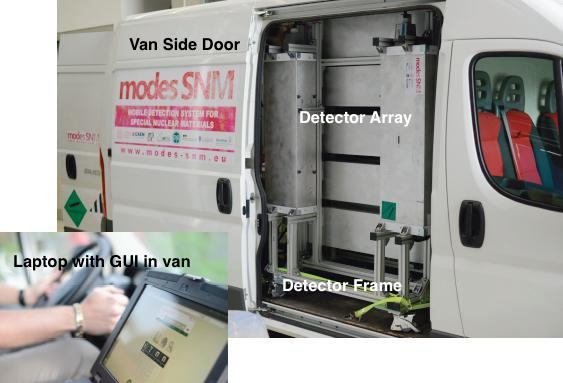
\includegraphics[width=125mm]{./Chapter7/figures/MODESsetup.jpg}
\end{center}
\caption{The MODES system setup in the van.}
\label{fig:modesSetupInVan}
\end{figure}

\section{Software Interface}
The MODES prototype is operated and monitored through a software interface which is accessible via any device with a wireless connection. Devices such as laptops and smartphones can connect to the Graphical User Interface (GUI) at a distance of up to 20 m from the van, shown in figure \ref{fig:modesSoftwareInterface}. 

\begin{figure}
\begin{center}
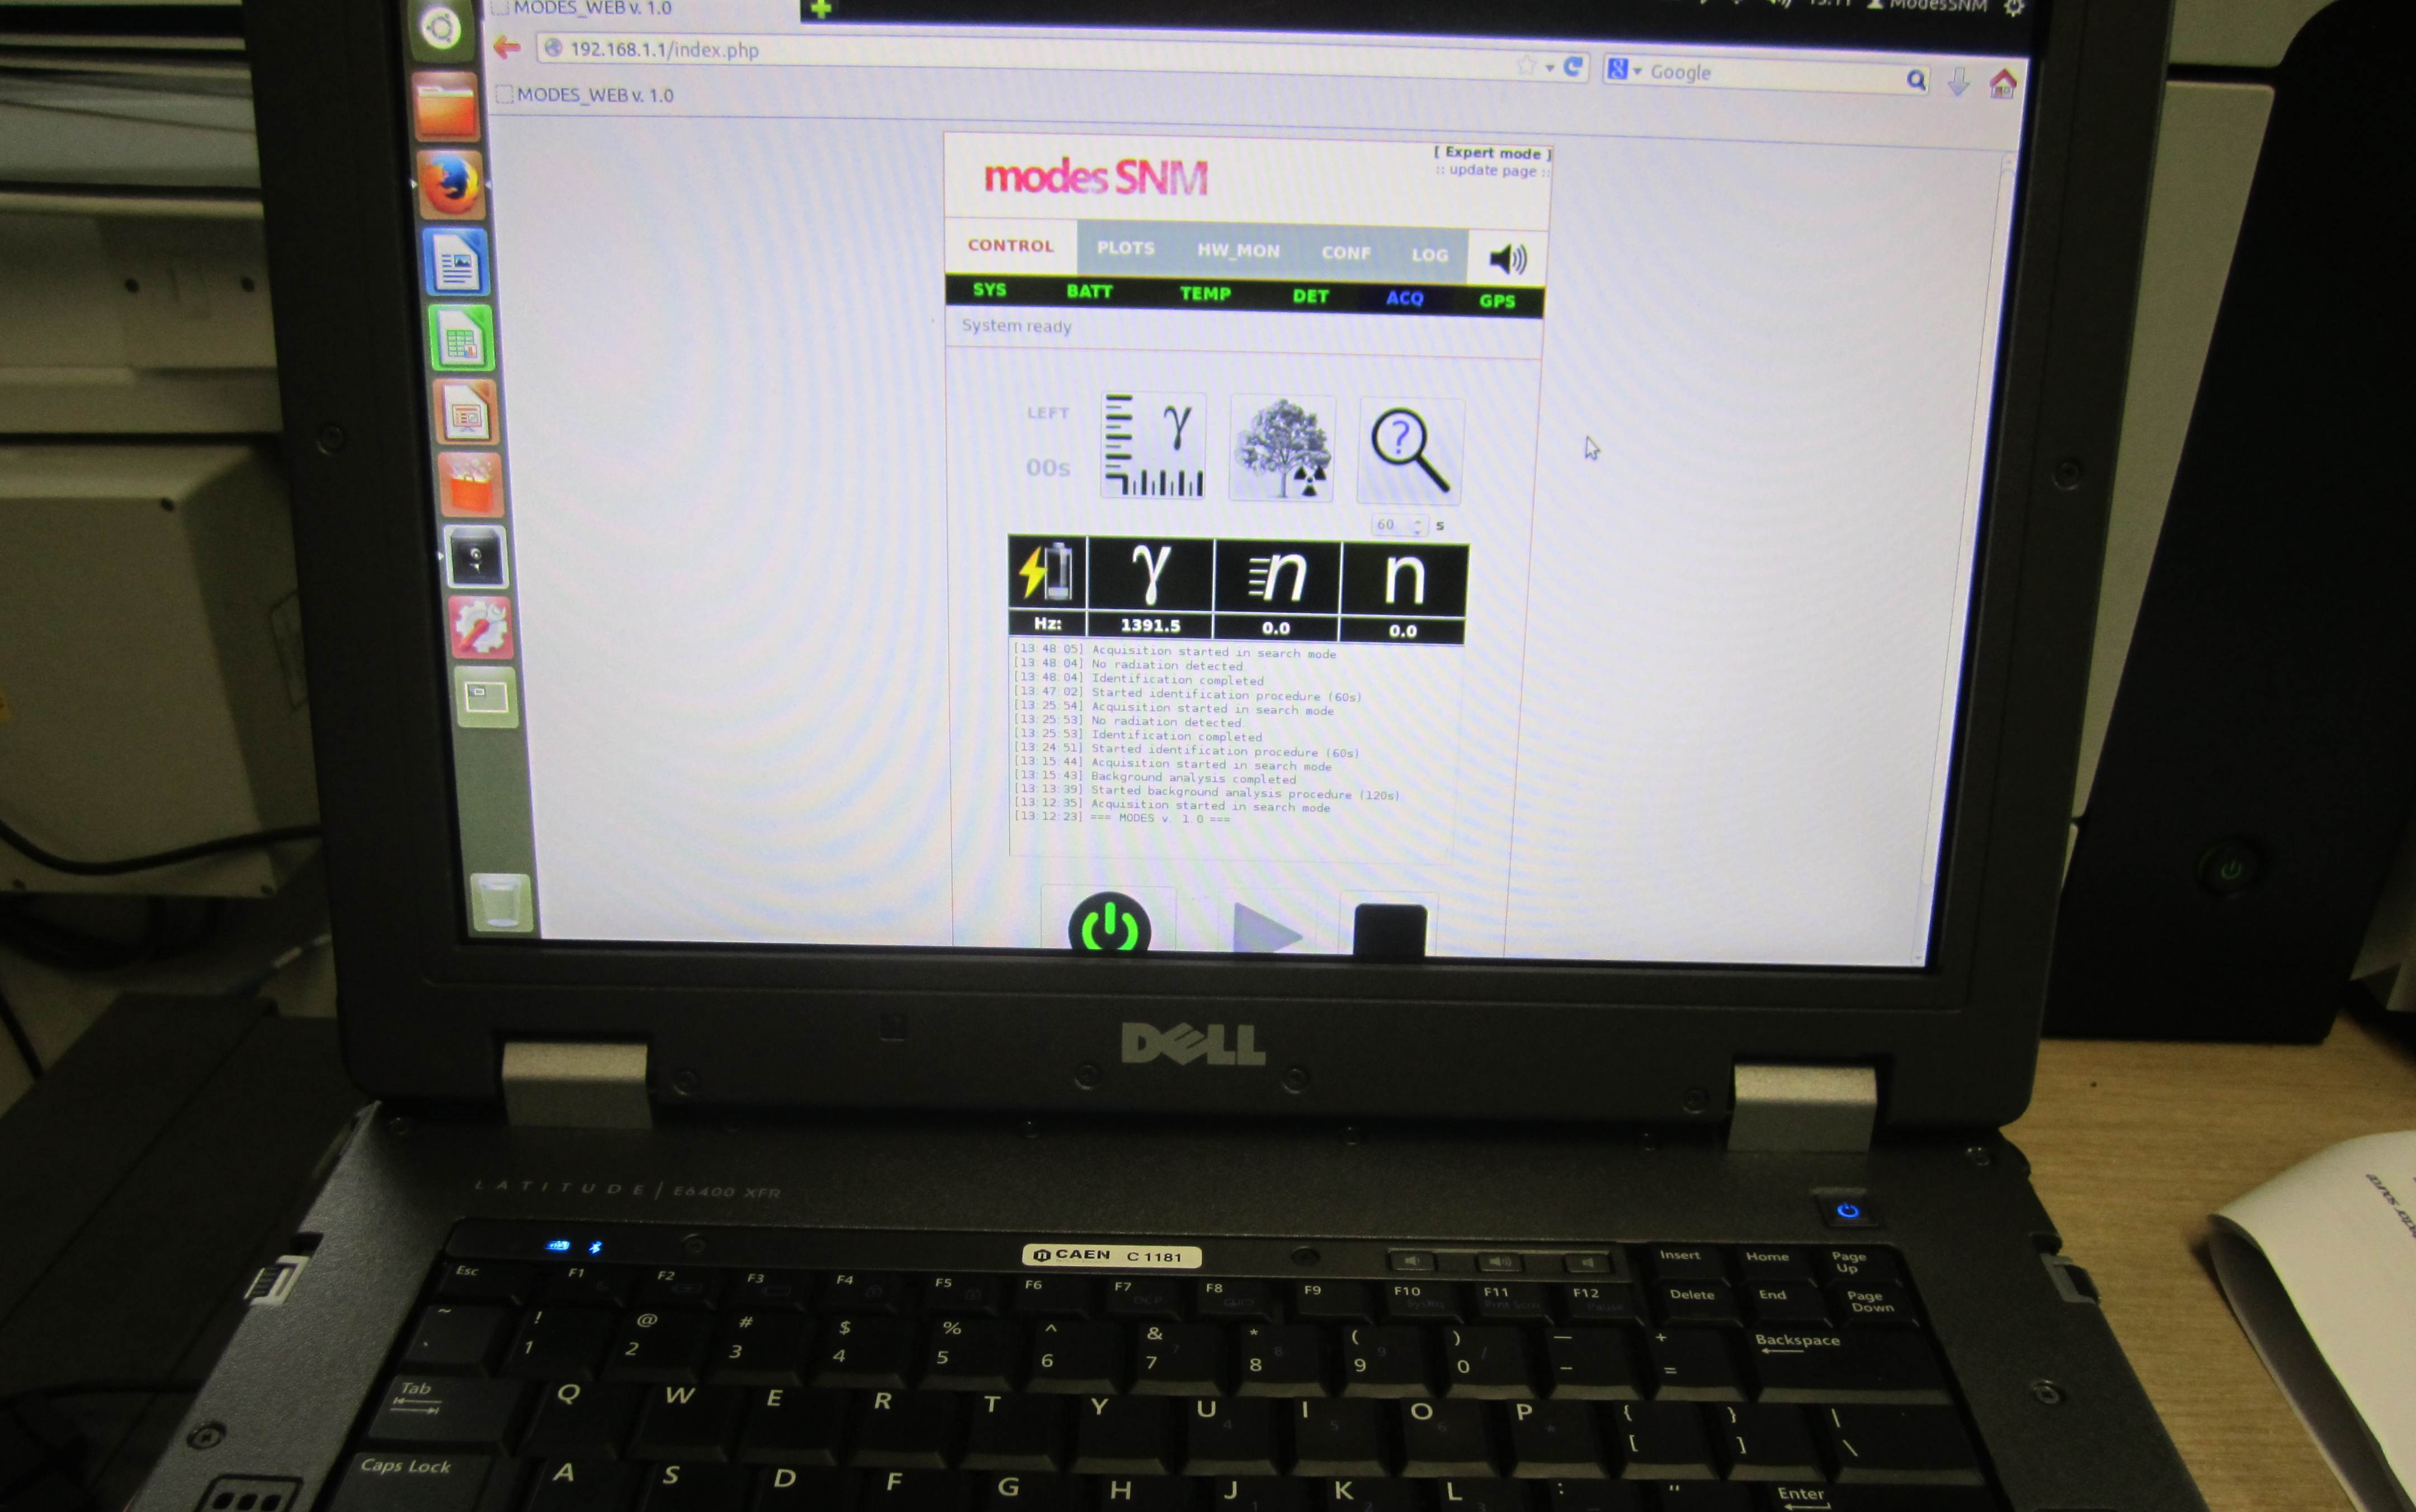
\includegraphics[width=155mm]{./Chapter7/figures/laptop.jpg} \\
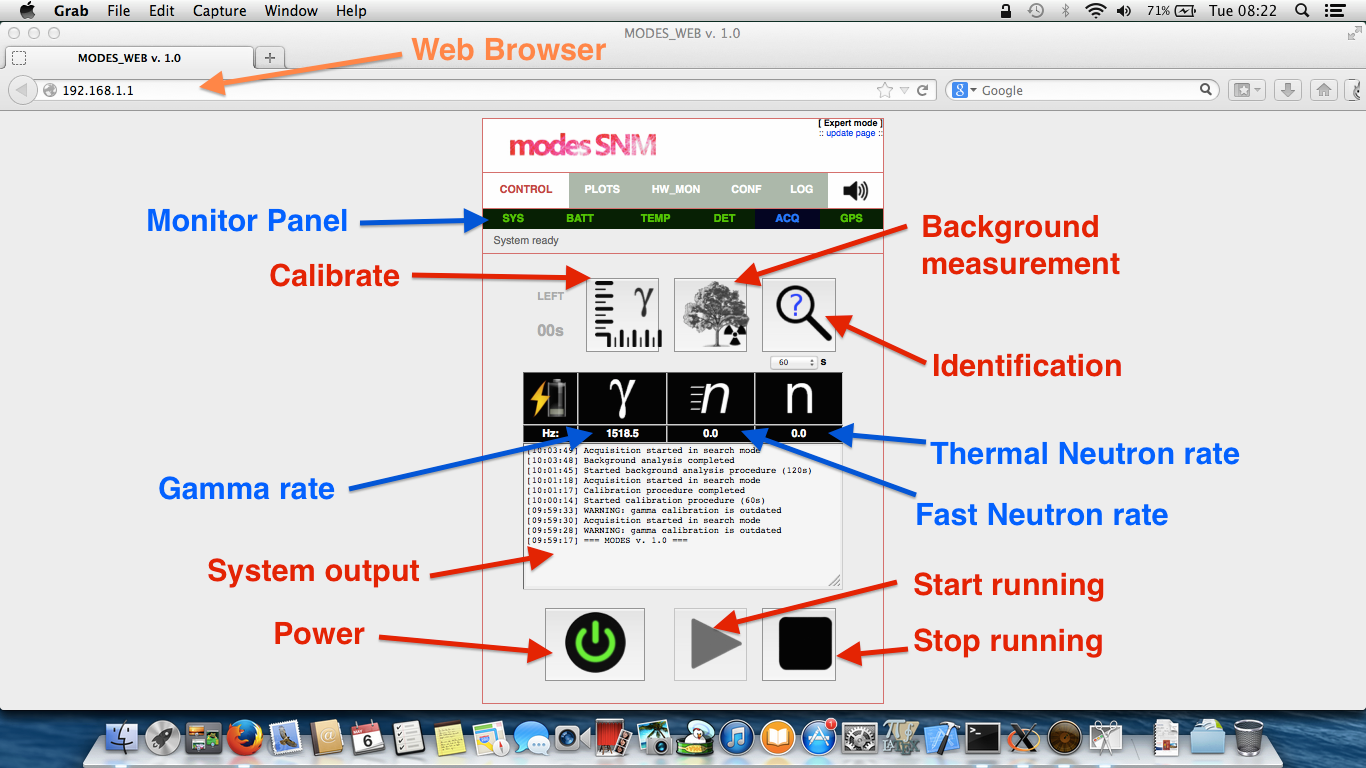
\includegraphics[width=155mm]{./Chapter7/figures/softwareInterfaceMainPage.png}
\end{center}
\caption{Top: The software interface show on a laptop. Bottom: The control page of the software shown in an internet browser with labels.}
\label{fig:modesSoftwareInterface}
\end{figure}

The software is accessible in two modes, normal and expert. Normal mode can only access the main control page, 'CONTROL' tab, which is shown in figure \ref{fig:modesSoftwareInterface} and is designed for users with no scientific background. This will be the default mode of operation and retains all functionality that an end user would need. The simplistic design of the interface is specifically tailored to such an end user with no background in nuclear physics. Expert mode should only be used as stated, by an expert, personnel who have substantial knowledge and understanding of nuclear radiation. In this mode energy spectra can be observed for each of the tubes in the detector array under the 'PLOTS' tab. Details on pressures, temperatures and voltages on the tubes are viewable under the 'HW$\_$MON' tab with these parameters configurable via the 'CONF' panel. An extensive log file is accessible, under the 'LOG' tab, which is far more heavily detailed than the one shown to the user in normal mode, showing energy spectrum peak values with corresponding $\chi^{2}/d.o.f$ values for fitting.

The procedure to start up the system and begin data acquisition is a simple 5 minute operation. With the battery connected to the electronics box the mechanical ignition key can be switched on and provide power to the whole system. Once the wireless connection has been established with the device used to control the system, in the case for demonstration this is the laptop, the user can then begin the procedure. A calibration run must first be performed, involving a 60 s exposure of a weak $^{60}$Co source (40 kBq) held close to the NaI detector via the coin sized slot on the side of the contatiner. Such a source is deemed safe to handle by a user and can be placed in the slot on the detector. Internal calibration is also continually performed but does not need interaction from the user. Following this a background measurement is then needed, which involves a 120 s exposure. The system output will print out details of the procedure to the user and notify when each step is completed. Upon completion of these steps the system is ready to begin data acquisition and is considered active. The various radiation rates: gamma, fast and thermal neutrons, are shown on the control page. 

\subsection{Energy Calibration}
For calibration of the MODES system two sources are used. One $^{40}$K source (1 kg KCl $\sim$32 kBq), is used internally in the NaI detector, which is continually present and the second is a $^{60}$Co source (40 kBq) that is used externally upon start up of the system. $^{40}$K emits a 1.46 MeV photon in around 10\% of decays via electron capture. The two peaks at 1.17 and 1.33 MeV originate from $^{60}$Co beta decay and then the subsequent nuclear de-excitation. These can be seen in the spectra when calibration is being performed figure \ref{fig:calibrationSpectra}.

\begin{figure}
\begin{center}
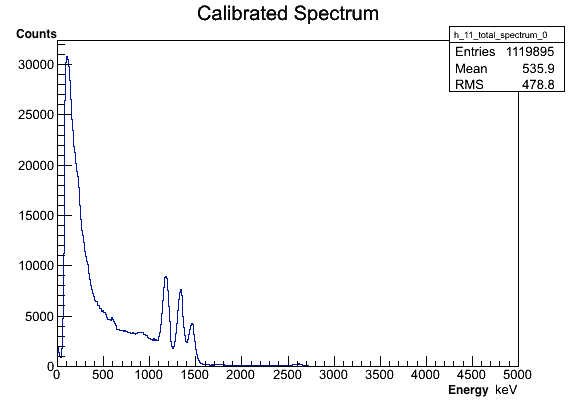
\includegraphics[width=75mm]{./Chapter7/figures/co60GammaCalibration.png}
\end{center}
\caption{The energy spectrum upon calibration as measured by the NaI detector.}
\label{fig:calibrationSpectra}
\end{figure}

\section{Joint Research Centre, Ispra Laboratory Tests}
Ispra Research Laboratories, located in Ispra, Italy, are one of Europe's leading research  facilities dedicated for experimental activities used for the development and testing of new technologies. It is then well suited to perform controlled laboratory tests on the MODES system. Such tests were performed at Ispra prior to the live demonstrations in order to test the system with SNM sources, as this would hopefully not be encountered at the demonstrations. Also it enabled the capability to test the system with known moving sources.

An IAEA requirement imposed on any potential radiation detection device is to raise a neutron alarm for a $^{252}$Cf source, of activity of 1.2 $\times$ 10$^{4}$ neutrons/s, whilst in motion at a speed of 0.5 m/s (1.8 km/h) \cite{modesIAEABorder}. It is also required that the distance between the source and the system $\geq$1 m. This is equivalent to a static rate of 0.1 neutrons cm$^{-1}$s$^{-1}$ at 1 m distance. Such tests successfully met this requirement with the results shown in table \ref{tab:IspraCfResults}. Other neutron sources were also used to test the neutron detection capabilities, all conducted at the speed of 1.8 km/h, table \ref{tab:IspraNeutronResults}.

\begin{table}[!htbp]
\begin{center}
	\begin{tabular}{l*{3}{c}r}
	\hline
	 \hline
	 Speed & Alarms & Trials & Success Rate\\
    	\hline
   	km/h & - & - & \% \\
    	\hline
    	\textbf{1.8} & \textbf{30} & \textbf{30} & \textbf{100.0} \\
    	4.3 & 28 & 30 & 93.3 \\
    	7.9 & 23 & 30 & 76.7 \\
    	\hline
    	\hline
  	\end{tabular}
	\caption{The speed tests for a $^{252}$Cf source (1.2 $\times$ 10$^{4}$ n/s) at 1 m distance performed at Ispra}
    	\label{tab:IspraCfResults}
\end{center}
\end{table}

\begin{table}[!htbp]
\begin{center}
	\begin{tabular}{l*{2}{c}r}
	\hline
	 \hline
	 Source & Alarms & Trials \\
    	\hline
    	AmBe 						 			& 10 & 10 \\
    	AmBe shielded 1cm lead + 1 cm iron 			& 10 & 10 \\
	Am/Be shielded 1cm lead + 1 cm iron + 8 cm poly 	& 10 & 10 \\
	Pu (6 g - 61\% enriched in $^{239}$Pu)			& 5 & 5  \\
	Pu shielded 1cm lead + 1 cm iron				& 5 & 5  \\
	Pu shielded 1cm lead + 1 cm iron + 8 cm poly		& 5 & 5 \\
	$^{252}$Cf 1cm lead + 1 cm iron + 8 cm poly		& 5 & 5 \\
    	\hline
    	\hline
  	\end{tabular}
	\caption{Various neutron sources used to test the MODES system in laboratory conditions with a separation of 1 m from the detector.}
    	\label{tab:IspraNeutronResults}
\end{center}
\end{table}

The IAEA also impose a requirement for the dynamic sensitivity of gamma radiation such that the system shall generate an alarm for $^{241}$Am, $^{137}$Cs and $^{60}$Co sources whilst in motion at a speed of 0.5 m/s (1.8 km/h) \cite{modesIAEABorder}. Once again the distance of closest approach should be no less than one meter between the source and the detection system. The gamma results met this requirement and are shown in table \ref{tab:IspraGammaResults}. Given the variable activities of the sources, the distance of closest approach was varied in order to compensate. Identifications were also performed on the sources in a 60 s exposure while probing in stationary mode. Ten attempts at identification were performed on each with each attempt successful.

\begin{table}[!htbp]
\begin{center}
	\begin{tabular}{l*{3}{c}r}
	\hline
	 \hline
	 Source & Dose Rate & Speed & Alarms/Trials \\
    	\hline
   	- & nSv/h & km/h & - \\
    	\hline
    	$^{60}$Co	 & 50 & $\leq$7.9 & 30/30 \\
    	$^{133}$Ba & 10 &$\leq$7.9 & 30/30 \\
    	$^{241}$Am & 50 & 1.8 & 30/30 \\
    	$^{241}$Am & 50 & 4.3 & 20/30 \\
    	\hline
    	\hline
  	\end{tabular}
	\caption{Various gamma sources used to test the MODES system in laboratory conditions.}
    	\label{tab:IspraGammaResults}
\end{center}
\end{table}

\section{London Heathrow Airport Demonstration}
London Heathrow International airport is the busiest airport in the UK, with an average of $\sim$1200 aircraft movements daily. In 2013 the cargo tonnage passing through the airport reached over 1.4 million tonnes \cite{heathrowStats}. It is therefore a perfect environment to perform field tests for the prototype system.

The UK Border Force (UKBF) are responsible for monitoring all cargo that is imported and exported via Heathrow. However only shipments for import into the airport are scanned for radiation. All cargo is loaded on to vehicles, consisting of vans and trucks, to be transported around the airport. Every vehicle must first pass through a control area at the airport, where it is scanned, before it is fit for import. 

\subsection{Current System and Procedure}
At the entrance to the control area, a large RPM is mounted, this is the UKBFs primary radiation detection system, shown in the left of figure \ref{fig:detectorsAtHeathrow}. If the RPM is triggered when a truck is passing, an alarm is raised via lights and a siren. The vehicle in question is then stopped and guided to an examination area for further investigation. Upon examination of the vehicle, the UKBF use secondary detectors, identiFINDERs (produced by FLIR) \cite{identifinderFlir}, shown in the right of figure \ref{fig:detectorsAtHeathrow}, to help identify the source of radiation. The identiFINDER uses NaI detectors to identify gamma radiation sources, with optional $^{3}$He detectors to detect neutron radiation. 

%Similar to the MODES system, the RPM has the ability to record the radiation count rate as a function of time.
The RPM has a laser tracking system, used to trace out the vehicle outline as it passes the detectors. Coupled with the measurement of the count rate with time, gives the user the ability to localise the source position on the truck, within a distance of around a meter. With cargo containers of the order of a 1 m in length this can help deduce which container is the cause for concern. From this information the secondary inspection device, the identiFINDER, can be used more successfully, homing in on the source. 

On secondary inspection the count rate is measured and an identification is performed. If the count rate is considered safe and the source identification matches the corresponding documentation for the cargo, the cargo is suitable for import and released from the control area. However if an identification proves inconclusive or yields an unknown source after repeated measurements, then external advice is required. A Radiation Protection Advisor (RPA) is an external entity that has expert knowledge on radiation and is called upon when the system fails to identify the source correctly. It is then up to the RPA to decide the fate of the cargo given data and information from the RPM software, including energy spectra and rates.

%RPM pictures
\begin{figure}
\begin{center}
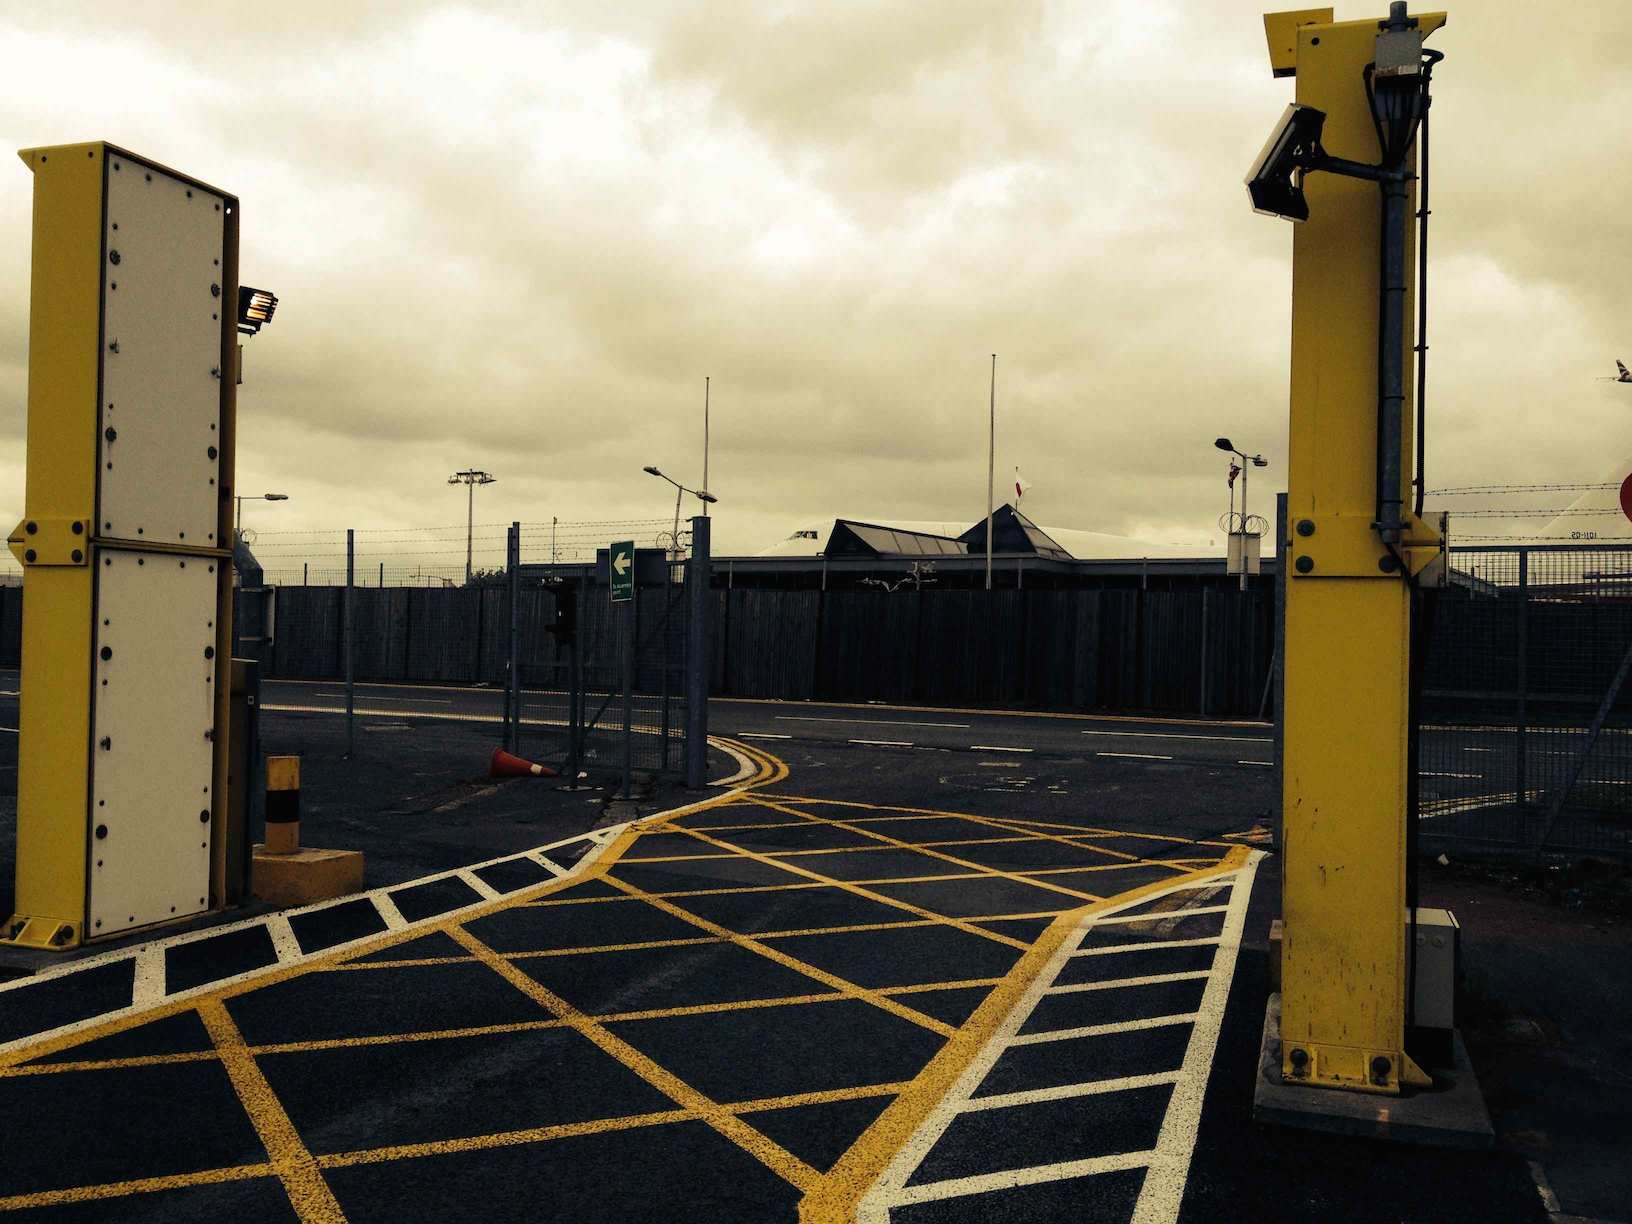
\includegraphics[width=75mm]{./Chapter7/figures/rpm1.png}
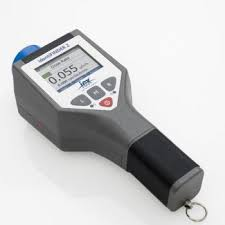
\includegraphics[width=75mm]{./Chapter7/figures/identiFINDER.jpg}
\end{center}
\caption{Left: The RPM in use at Heathrow Airport to scan and monitor all shipments arriving for import. Right: The identiFINDER, produced by FLIR, used for secondary investigation after the RPM alarm is raised}
\label{fig:detectorsAtHeathrow}
\end{figure}

\subsection{Setup}
The van is setup with the detector array facing the road upon which the cargo vehicles travel. At this position the typical distance between the MODES van and the passing traffic is no more than 1.5 m and in operation the door is left open.

\begin{figure}
\begin{center}
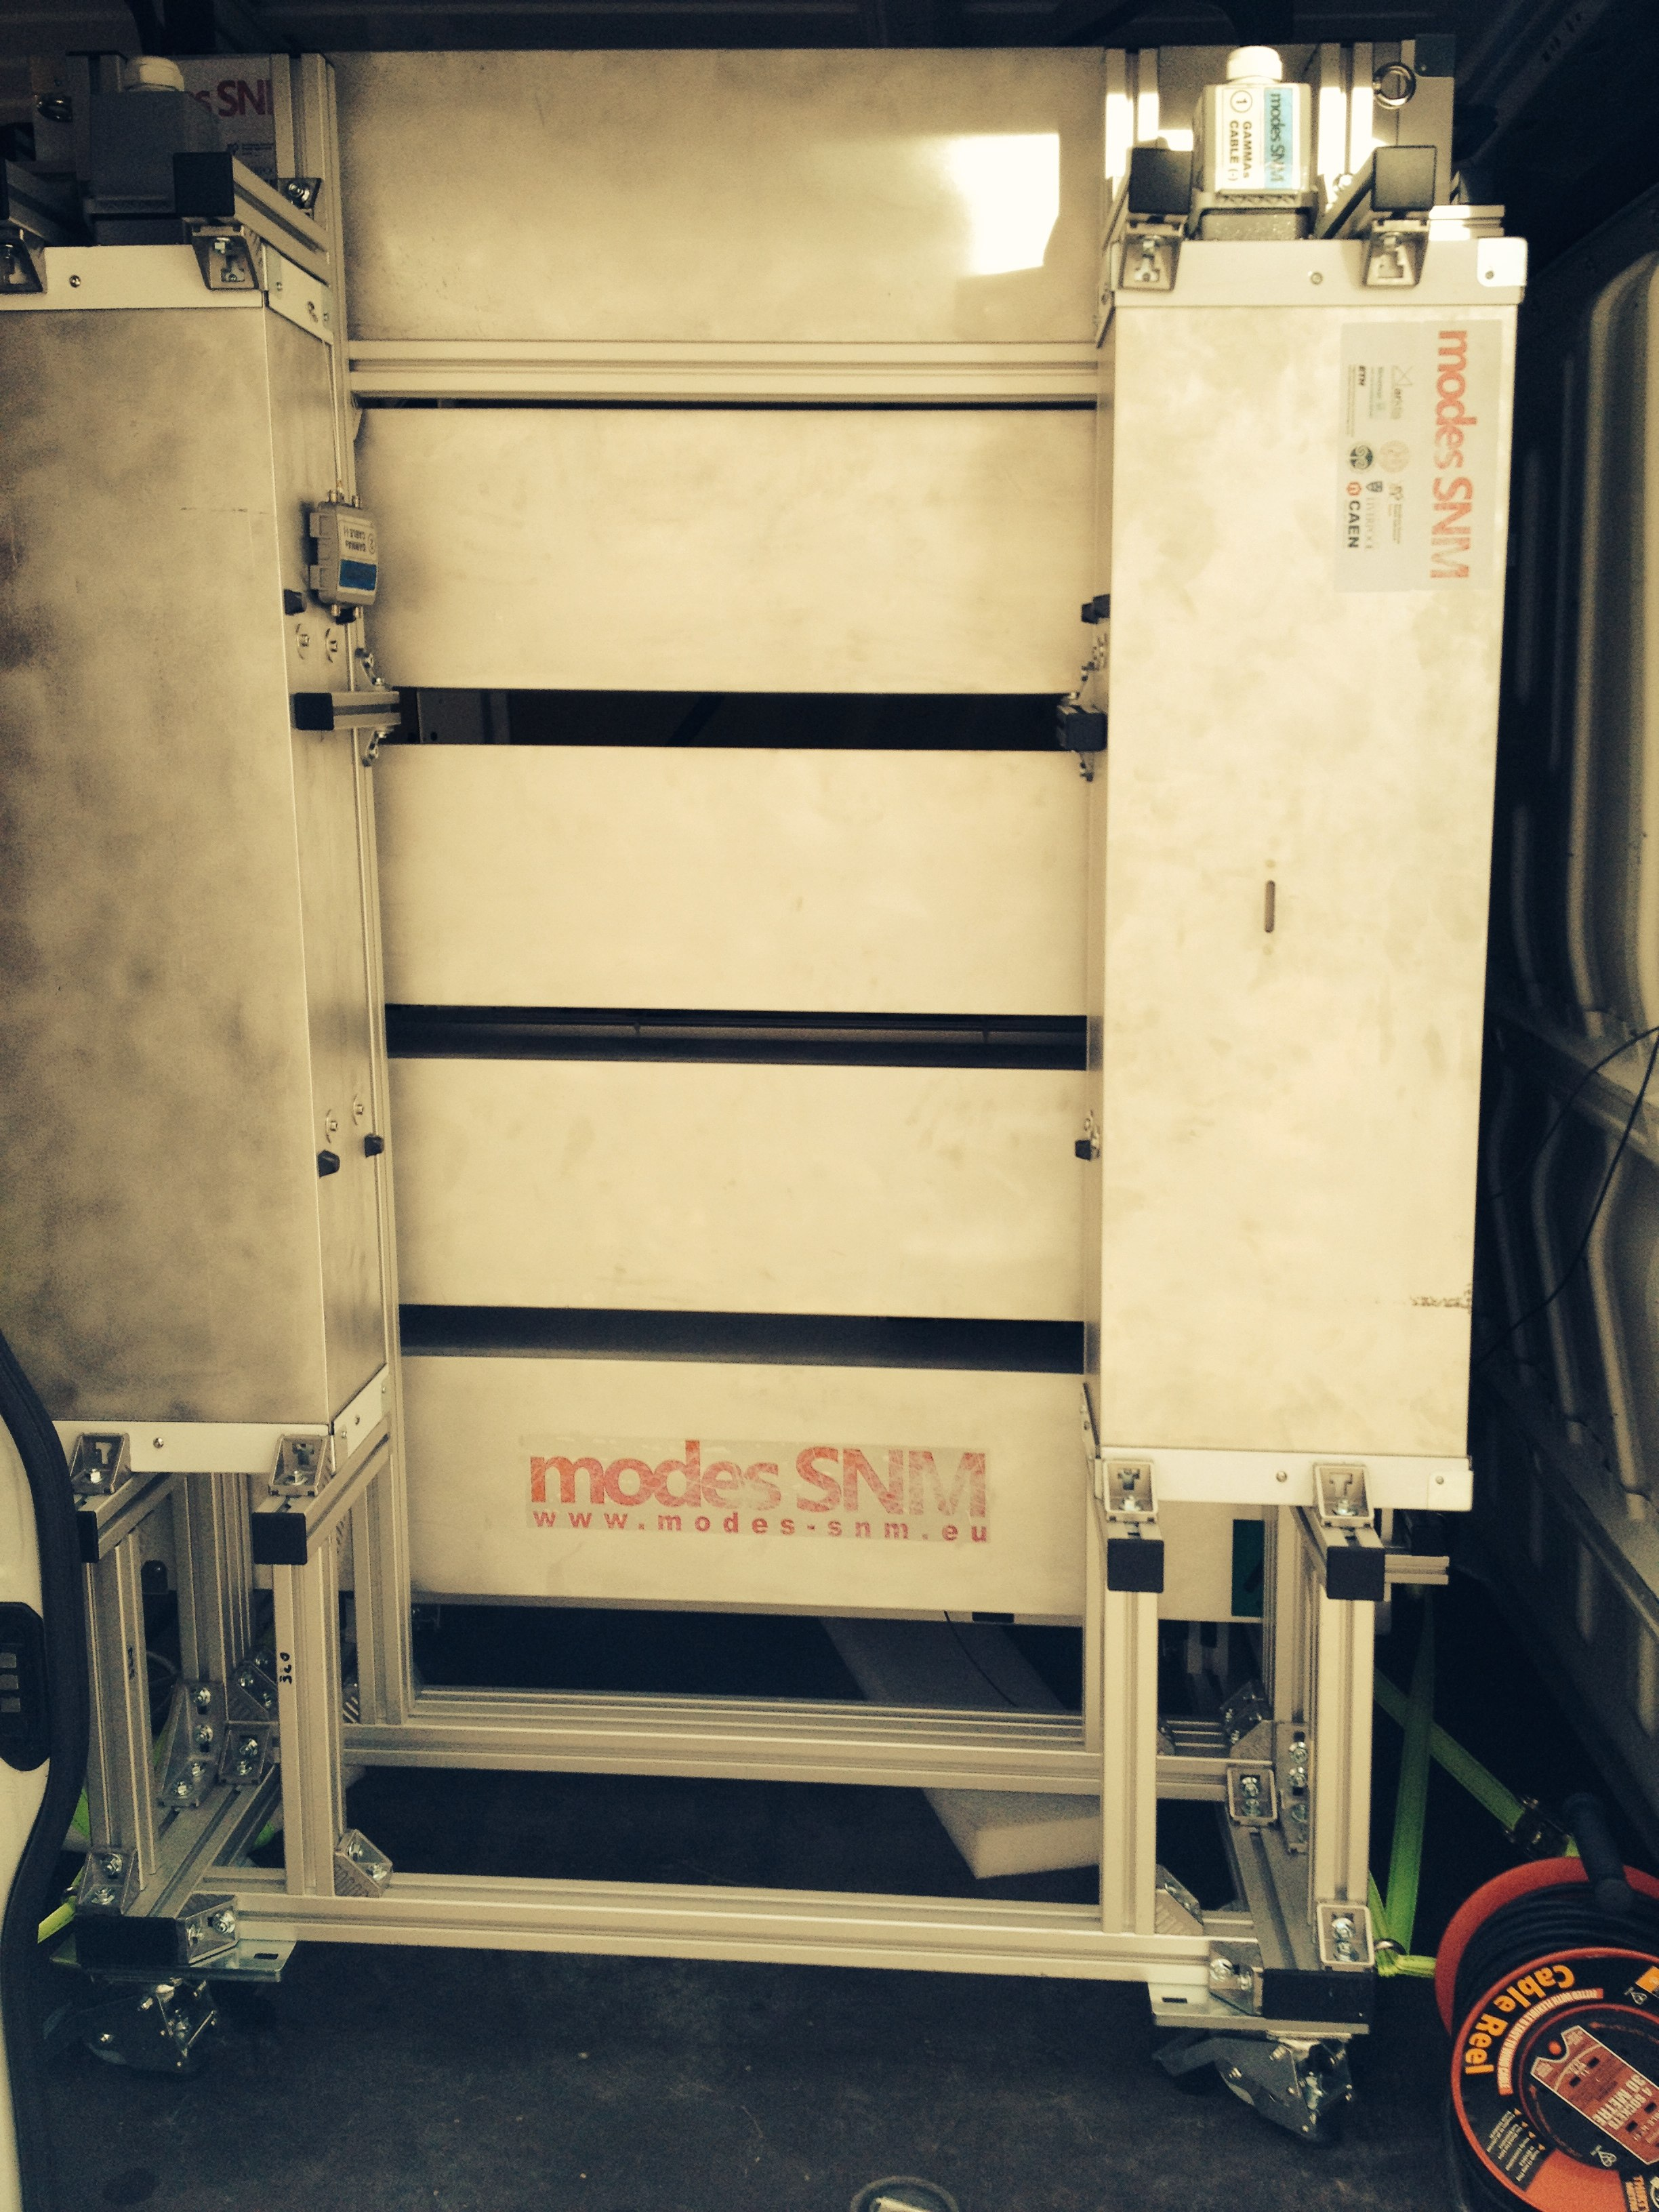
\includegraphics[width=75mm]{./Chapter7/figures/detectorArrayInVan.jpg}
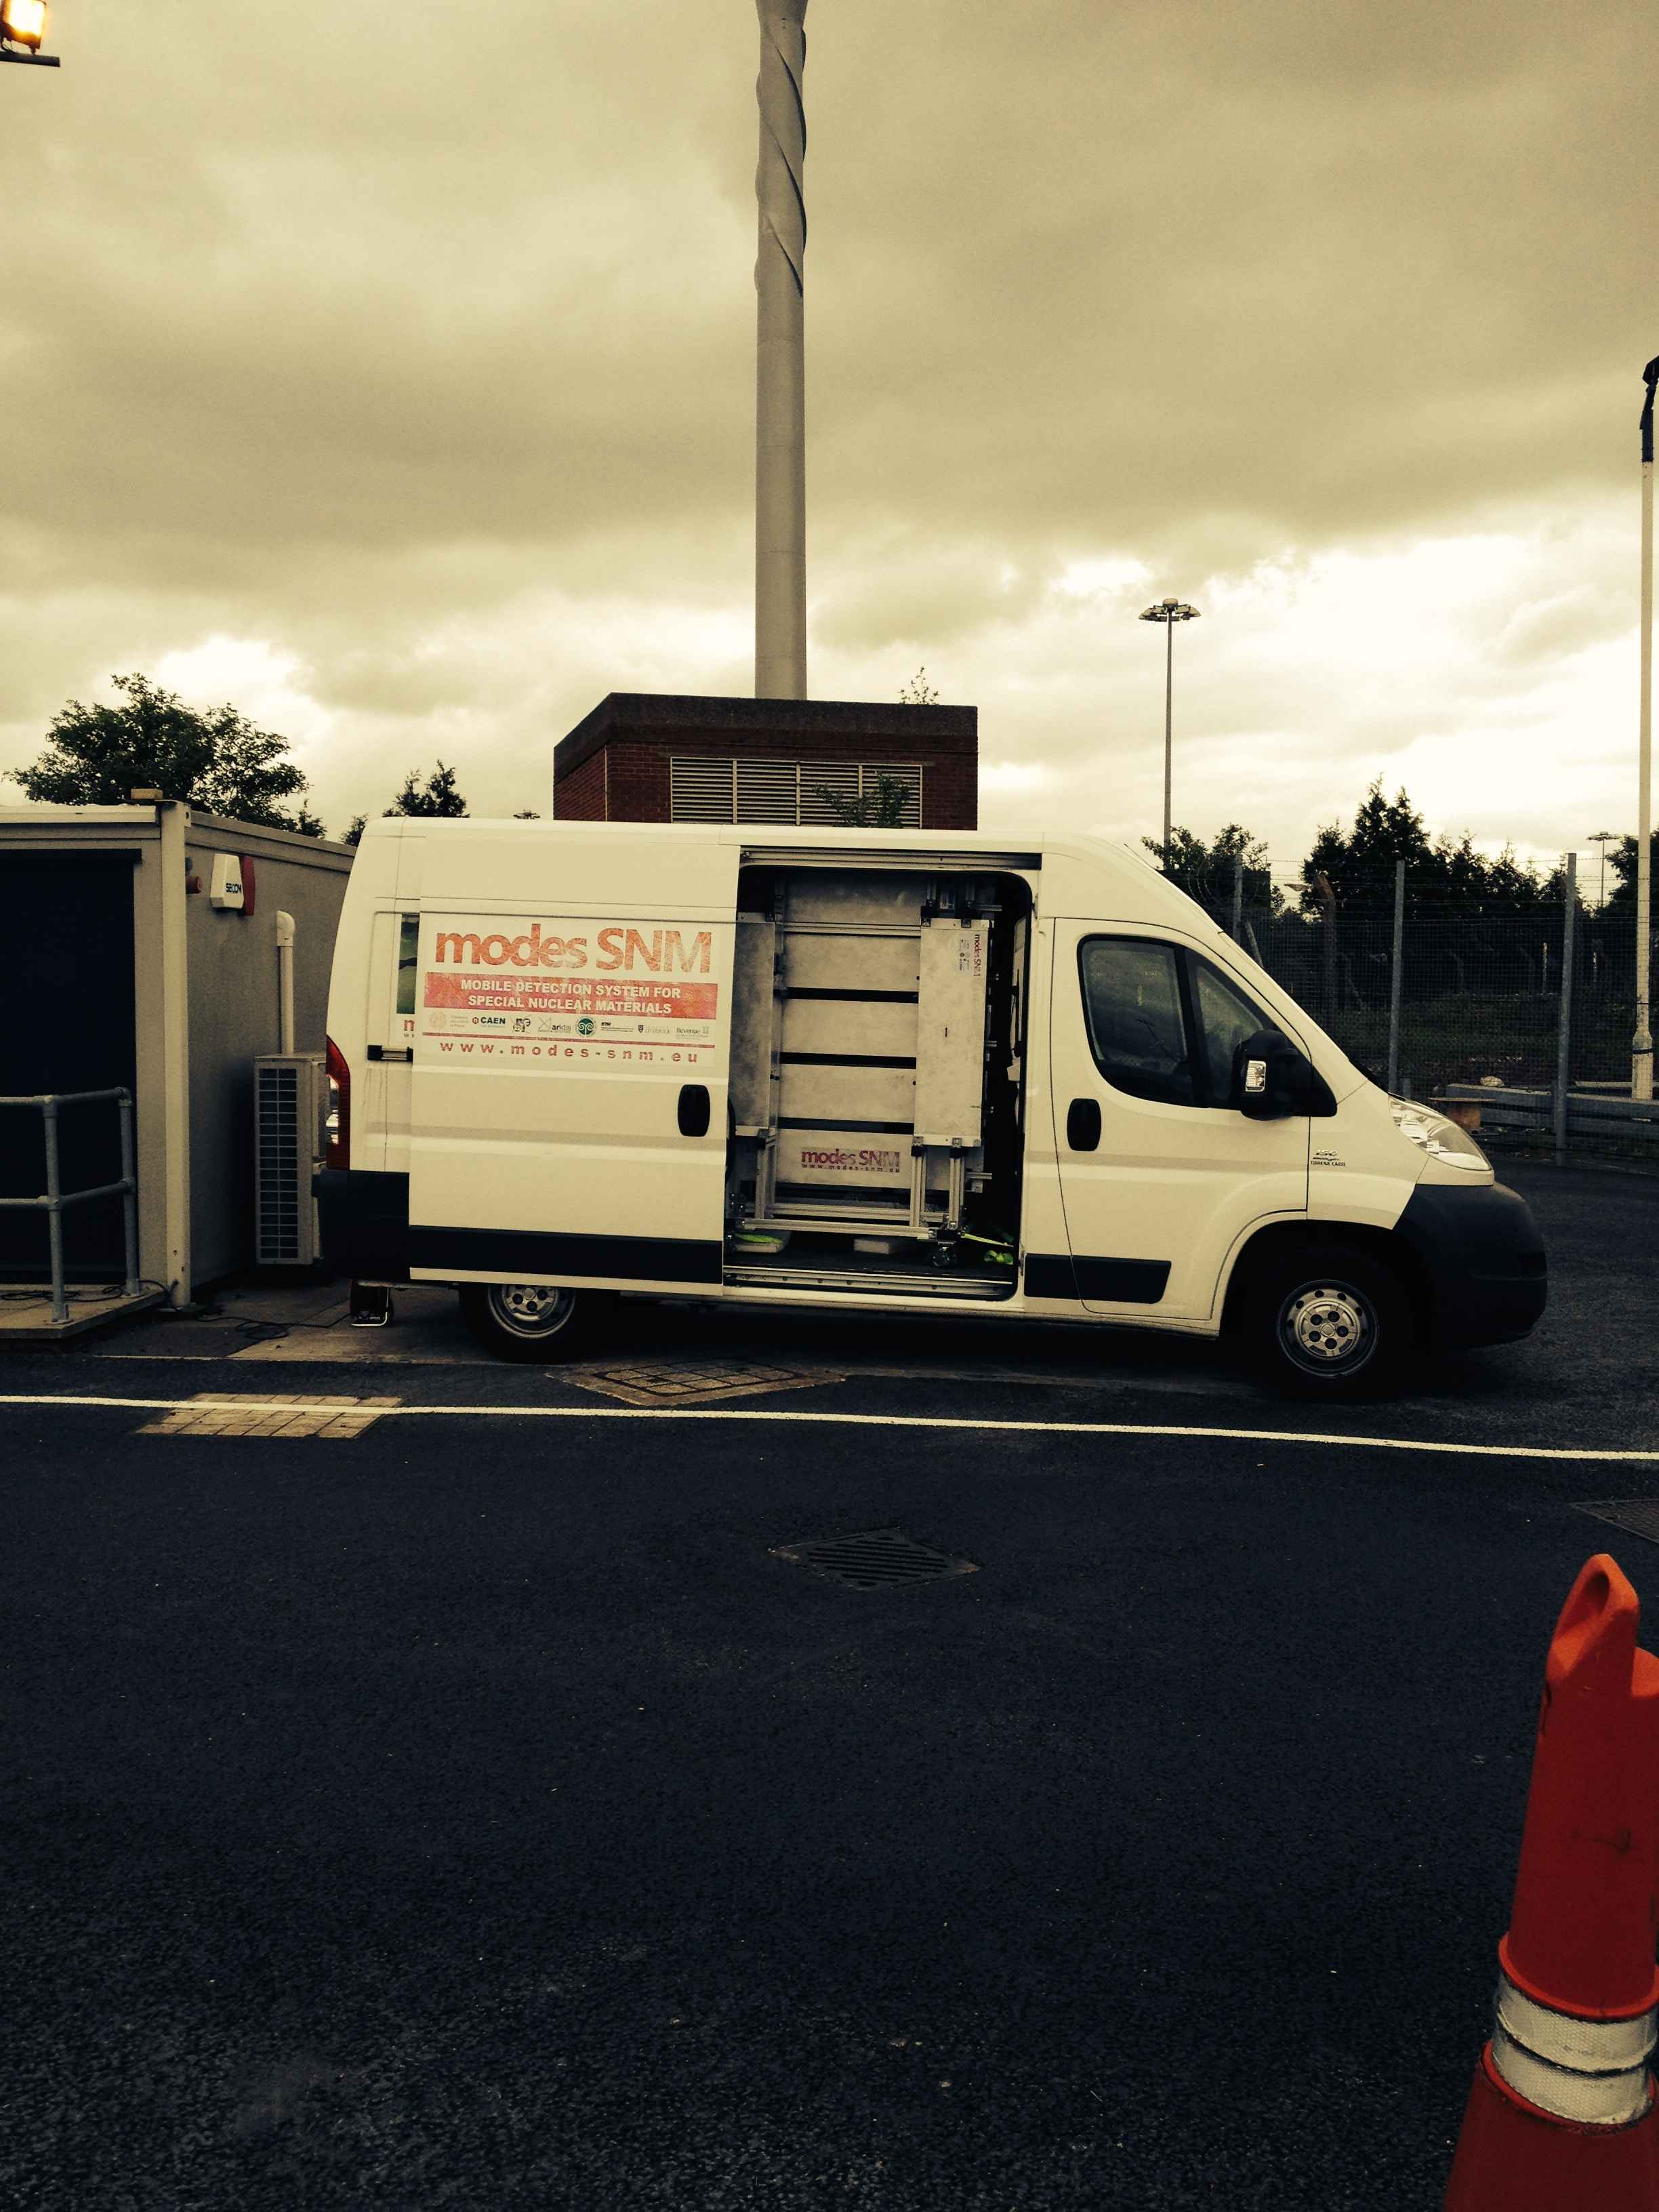
\includegraphics[width=75mm]{./Chapter7/figures/modes_van1.jpg}
\end{center}
\caption{The MODES system mounted in a medium wheelbase van. Left: The detector array mounted on the frame. Right: The MODES van with the side door open to expose the detector array.}
\label{fig:modesVanHeathrow}
\end{figure}

\subsection{Stationary Mode - Passing Vehicle Testing}
While the system was operational in stationary mode for testing passing cargo, a total of 635 vehicles passed the system, covering a 20 hour period. From these passing vehicles one false positive alarm and one true positive alarm occurred only. Many gamma alarms occurred also when no vehicles were present, with an average of 3 alarms per hour, totalling to $\sim$60 such incidents. These occur due to a low threshold setting in the system and fluctuations in the background can trigger such alarms. Although no vehicles were present, future designs and upgrades for the system must consider removing these alarms if the system is to survive the scrutiny from potential buyers.

\subsection{False Positive Alarm}
On the second day of testing, after 140 vehicles had already passed the system without an alarm, a false positive alarm was raised by a passing vehicle. The alarm was short and the gamma count rate was similar to the background rate of $\sim$1400 Hz, initially raising suspicion that this may a false positive. However following procedure the vehicle was instructed to stop at the examination area for further probing. At a distance of 0.5m from the vehicle MODES failed to pick up any signs of radiation after repeated measurements of exposures from 60 to 300 seconds. The gamma count rate decreased upon approach to the vehicle to a value $\sim$ 1100 Hz, due to vehicle shielding. The identiFINDER also failed to detect any radiation. Cargo itinerary revealed oil mining equipment which is fit for transport and not a radiation threat. The vehicle was subsequently released. 

It was a displeasing result and highlights that the sensitivity of the system is an issue as it increases the number of false alarms. The probability of such an event occurring due to background fluctuations is much smaller than observed however. As in the 20 hour period 635 vehicles passed the detector, with each taking $\sim$6-8 s to fully pass the van. Hence on average $\sim$6\% of the time a vehicle was present. With an average of 3 alarms raised when no vehicles were present per hour, but with a maximum of 4 per hour, and each lasting $\sim$2 s, yields an upper limit that $\sim$0.2\% of the time an alarm is triggered by the background. For these two events to both occur results in $\sim$0.014\% probability, which would mean we can expect 1 false alarm for every $\sim$7,400 passing vehicles. Thus from the 635 vehicles observed we would expect 0.09 false alarms while a vehicle is present but we observed 1 false alarm event. In terms of Poisson statistics an observation of one false alarm, with a mean of 0.09 false alarms, corresponds to P(n=1) = 8.2\% and P(n$\geq$1) = 8.6\% for one or more false alarms. Highlighting that this was quite an improbable occurrence but for large volumes of traffic this would not be acceptable and reasserts the need to lower the rate at which alarms are triggered from background fluctuations.

\subsection{True Positive Alarm}
On the fourth day of the demonstration, after a cumulative count of 319 vehicles passing MODES, the 320$^{th}$ such vehicle raised an alarm upon passing the MODES van. The vehicle was instructed to stop and moved to the examination area for further investigation. With the van parallel to the drivers side of the alarmed vehicle and at a distance of 0.5 m away, the van probed it while in motion at $<$8 km/h. Moving from the front to the rear of the vehicle the count rate increased sharply until a maximum of 7400 gamma counts s$^{-1}$ was reached near the centre. In comparison the background rate, at more than 10 m from the vehicle, was 1400 counts s$^{-1}$. After locating the maximum count rate position, a 60 s exposure led to an identification of a $^{60}$Co source on the first attempt. Repeated measurements yielded the same source with the peaks matched with a fit of $\chi^{2}/d.o.f$ = 0.198. The spectrum for a 2 s exposure can be seen in figure \ref{fig:cobalt60OnTruck}. 

\begin{figure}
\begin{center}
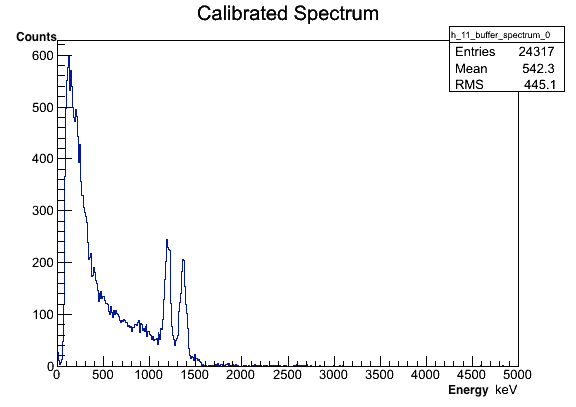
\includegraphics[width=100mm]{./Chapter7/figures/co60Gamma01Container060514-1120_2sExposure.png}
\end{center}
\caption{The energy spectrum of a $^{60}$Co source found on a cargo passing the MODES system for a 2 s exposure time. The two peaks at 1.17 and 1.33 MeV indicate $^{60}$Co.}
\label{fig:cobalt60OnTruck}
\end{figure}

The two peaks at 1.17 and 1.33 MeV, are a clear signature of $^{60}$Co. These occur following the beta decay of the isotope which leaves the daughter nucleus, $^{60}$Ni, in an excited nuclear state which subsequently emits two photons at these energies following from de-excitation. $^{60}$Co is not a naturally occurring isotope and is created artificially by the bombardment of neutrons on $^{59}$Co. The paperwork for the alarmed vehicle details that it contains two sources of $^{60}$Co of 500 kBq and 7.4 MBq, shielded by stainless steel. However other sources present of $^{137}$Cs (1.9 GBq) and $^{125}$I (activity not stated) were not picked up by the MODES system. $^{125}$I does not currently exist in the software spectrum library and could not be matched but $^{137}$Cs does exist in the library. $^{137}$Cs emits a 0.66 MeV photon 93.5\% of the time, but this is not seen in the spectrum in figure \ref{fig:cobalt60OnTruck}. This source may have been shielded much more than the $^{60}$Co and as a result cannot be identified. In terms of eligibility for transport the cargo ranks a category of Class 7, which label radioactive materials fit for transport. The vehicle was subsequently released.

This was a pleasing result and thoroughly impressed the UKBF. It was a perfect example of the sensitivity the MODES-SNM system possesses. 

\subsection{Container of Radioactive Sources at Heathrow}
At the control area a large container is used to hold confiscated radioactive sources that were not eligible for import. The sources in the container were known to the UKBF but a blind test was performed with the MODES van to see if it could identify any of the sources in the container. The sources in the container were: $^{60}$Co, $^{137}$Cs, $^{232}$Th and $^{222}$Rn. The alarm was raised initially at a distance of almost 10 m as the van approached the container. At 1 m away from the container with the detector modules facing the containers side, a gamma count rate in excess of 15000 Hz was observed ($\sim$11 times the background). Several exposures of 60 s correctly identified the $^{60}$Co source but failed to identify the remaining 3 sources. The activity of the sources is not known but the $^{60}$Co source originates from stainless steel bowls which were not classed as Class 7 on import. Isotopes $^{232}$Th and $^{222}$Rn could not be identified, with the 0.66 MeV photon from $^{137}$Cs not noticeable in the energy spectra, shown in figure \ref{fig:cobalt60Container}.

\begin{figure}
\begin{center}
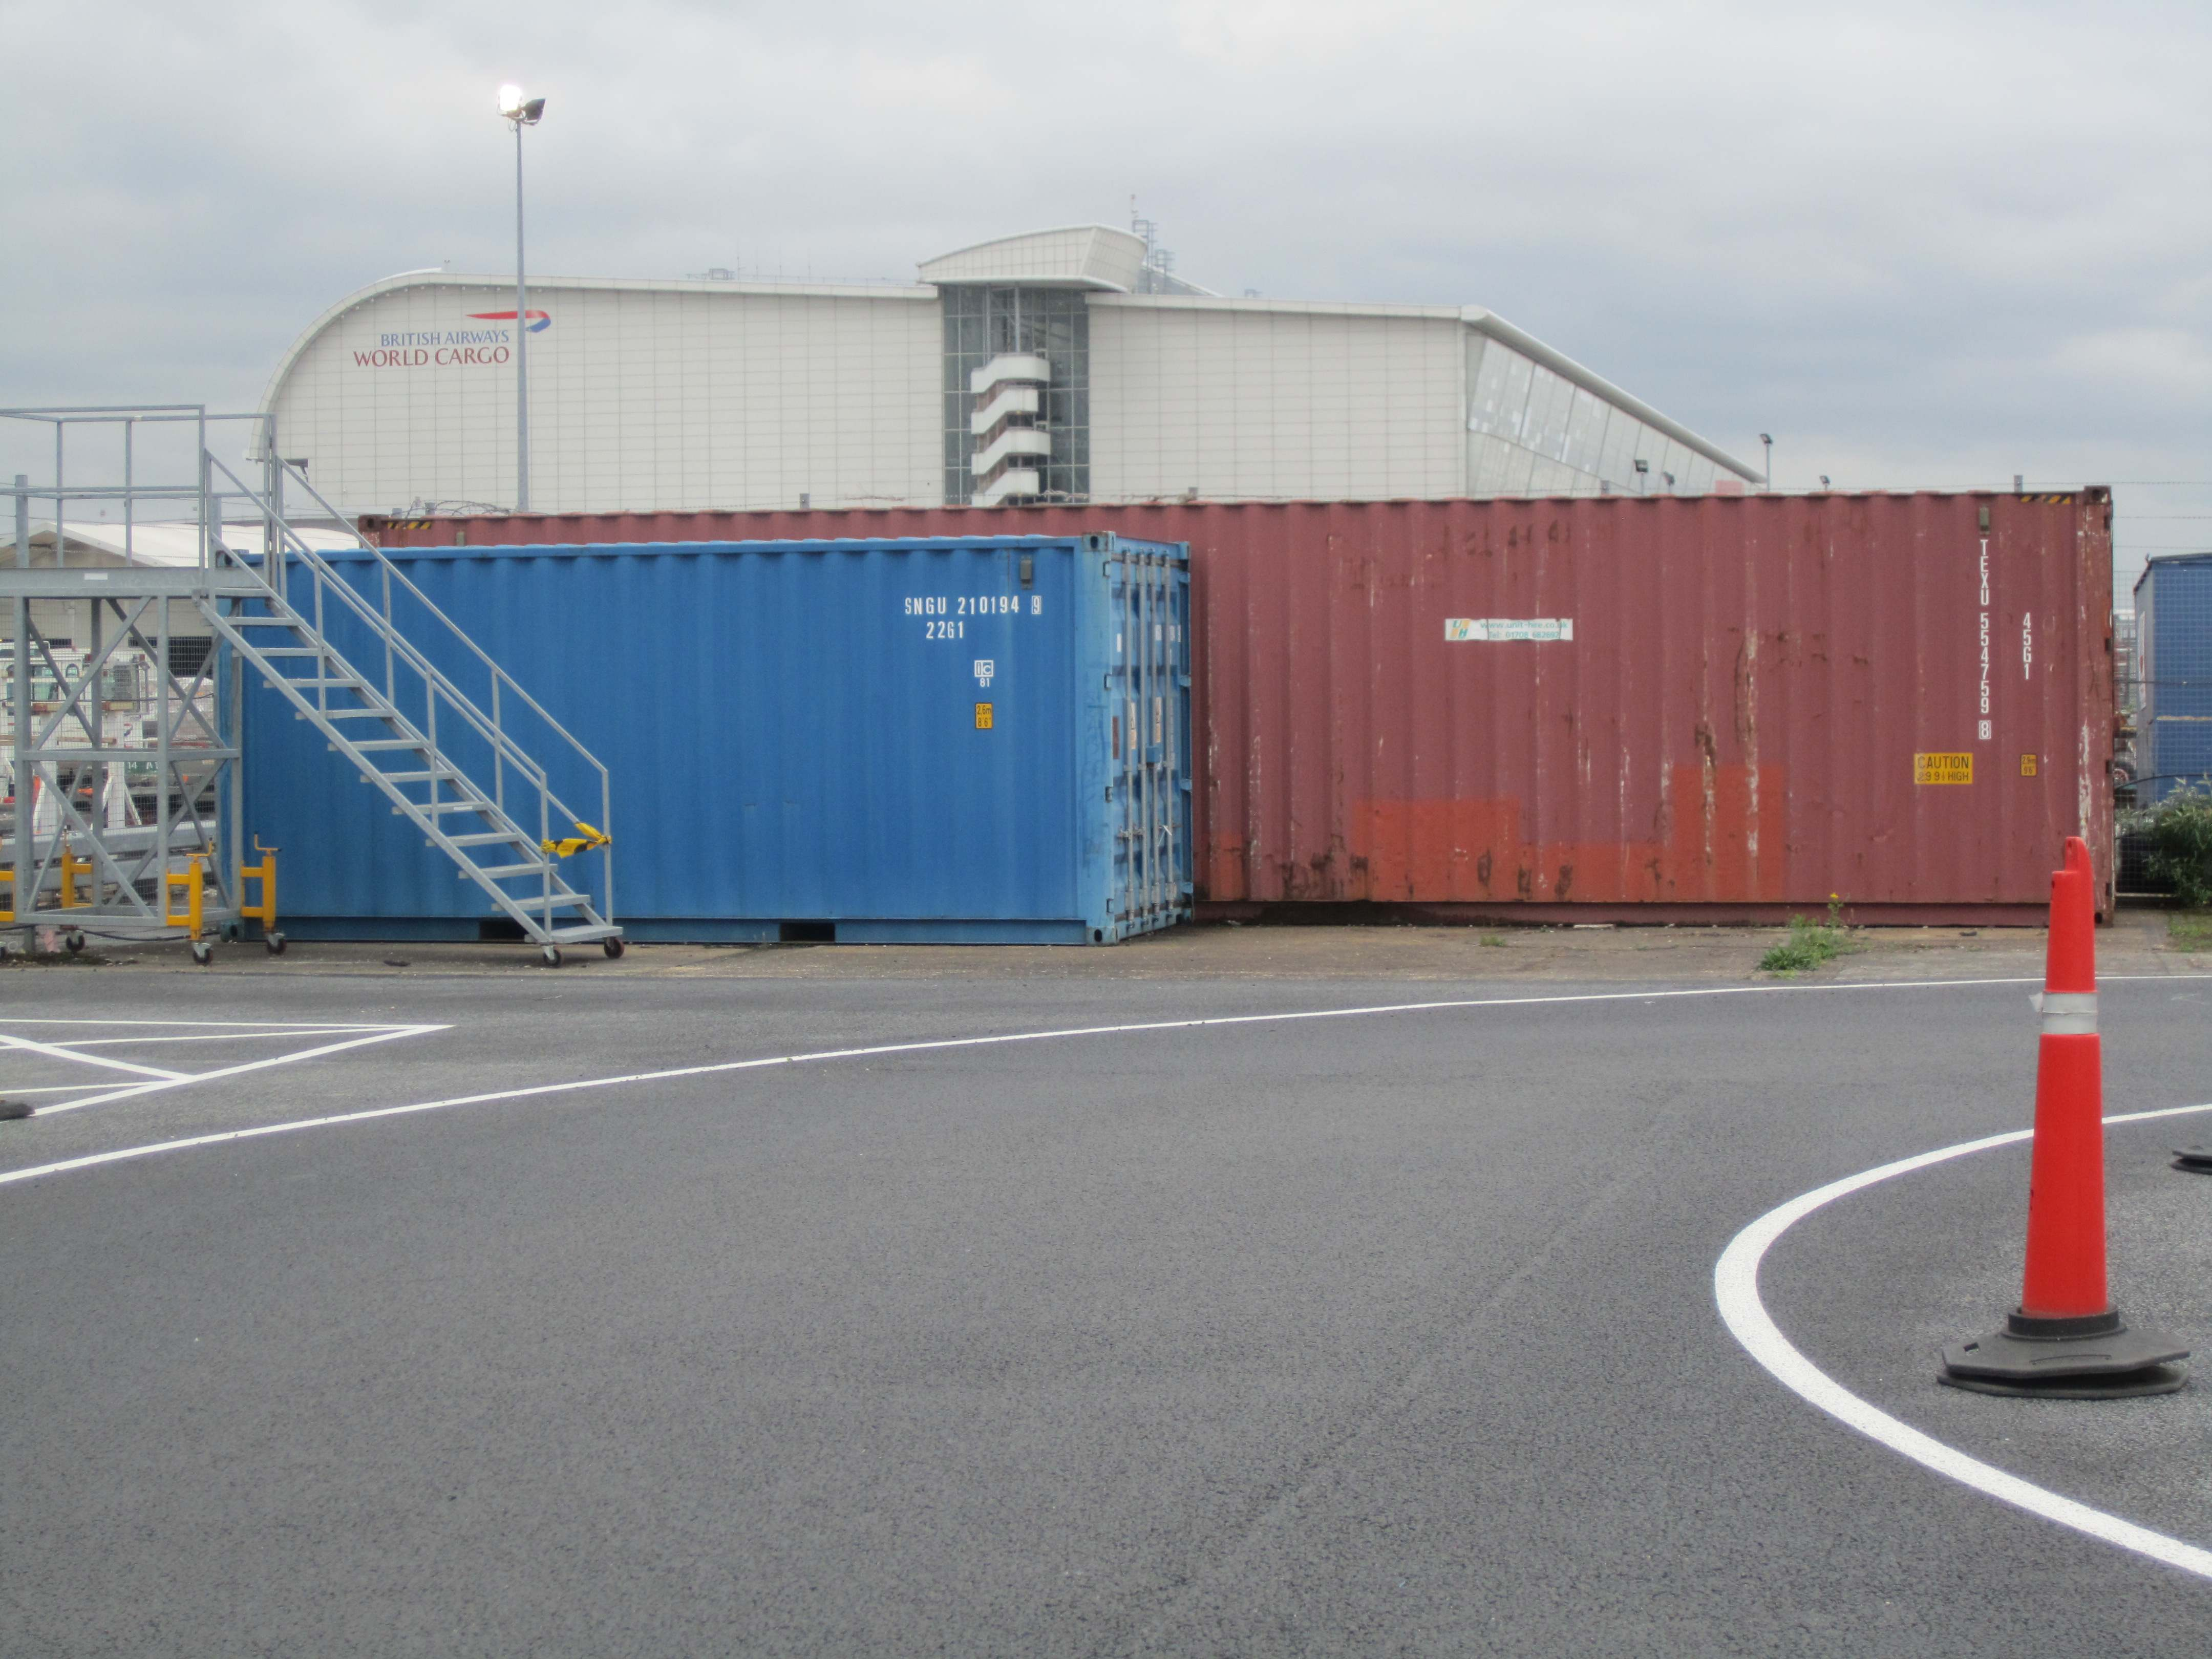
\includegraphics[width=75mm]{./Chapter7/figures/container.jpg}
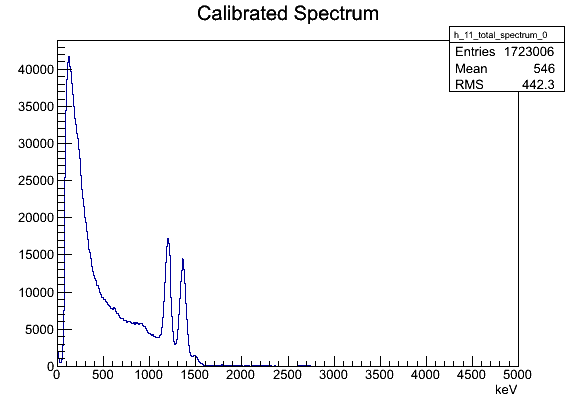
\includegraphics[width=75mm]{./Chapter7/figures/co60Gamma01Container060514-1120.png}
\end{center}
\caption{Left: A container holding various radioactive substances, of $^{60}$Co, $^{137}$Cs, $^{232}$Th and $^{222}$Rn, with the MODES van positioned along side it. Right: The energy spectrum from the container.}
\label{fig:cobalt60Container}
\end{figure}

Once again it was an impressive result, especially with the alarm raised at such a far distance from the source. The identification of $^{60}$Co was well received by the UKBF but of the sources found this was the most anticipated. The remaining sources were unidentified and it was a slight disappointment. It would of been productive to repeat the test without the $^{60}$Co source in the container and to then see if the remaining sources were identifiable, however it was not possible to perform such a test.

\subsection{System Stability and Reliability}
Over a period of five non consecutive days, the MODES system ran fully operational for the majority of demonstration. There were few minor problems with the system, with 3 software crashes in total, which were overcome with a simple laptop restart. Considering that the van had travelled over 2000 miles before arrival to Heathrow illustrates that the system fully fulfils the reliability requirement of the prototype while remaining mobile. 

\section{Other Demonstrations}
Other demonstrations were also performed at Rotterdam, Dublin and Switzerland, a summary is given for each.

\subsection{Rotterdam Port Demonstration}
The port of Rotterdam is the largest port in Europe and acts as a passage to the EU. On an annual basis more than 12 million cargo containers (Twenty-feet Equivalent Units based on 2014 statistics) pass through the port \cite{rotterdamStats}. The Dutch Customs are responsible for the scanning of such containers and detecting illicit radioactive and nuclear materials. They currently employ a range of fixed, mobile and hand held detection devices to aid them in this task.

Dutch Customs tested the MODES system in their daily use in the Port of Rotterdam. Similar procedures were employed at the port with trucks carrying cargo required to pass their primary detectors. Trucks that alarmed from the primary fixed RPMs were pulled over and investigated using secondary detectors. At ports large containers are common place and large lorries are required to transport them, seen in figure \ref{fig:rotterdamContainer1}, unlike Heathrow were cargo is held in much smaller volumes.

\begin{figure}
\begin{center}
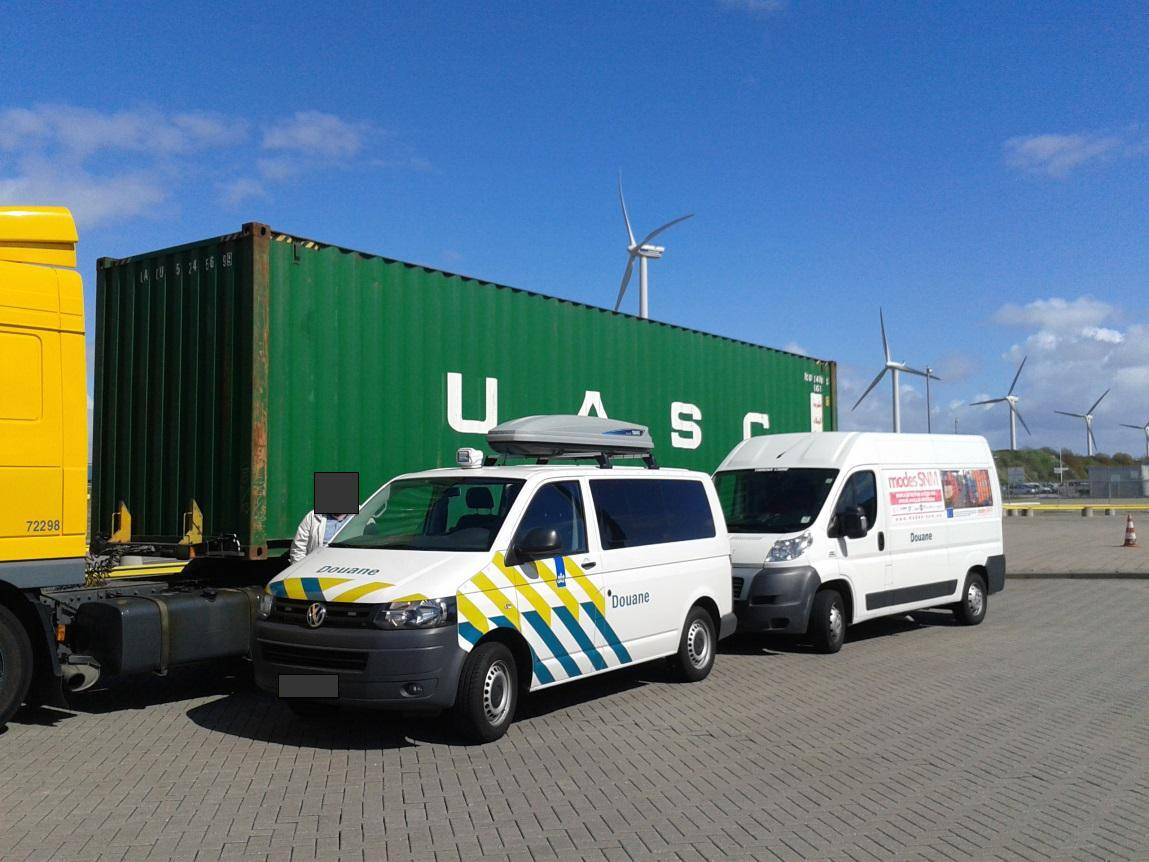
\includegraphics[width=75mm]{./Chapter7/figures/rotterdamContainer1.jpg}
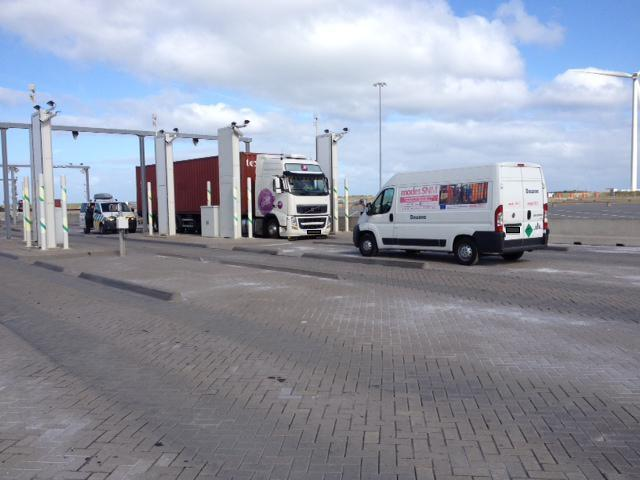
\includegraphics[width=75mm]{./Chapter7/figures/rotterdamRPM1.jpg}
\end{center}
\caption{Left: A typical lorry carrying a container under inspection with the MODES system and the currently used mobile system at the port by the Dutch Customs. Right: The truck passing the RPM at the port with the MODES system in front being used as a primary detector.}
\label{fig:rotterdamContainer1}
\end{figure}

The port experiences far more traffic than at Heathrow and as a result experiences many more alarms. Several different techniques were employed to fully test the MODES system. This consisted of MODES being deployed as a stationary and mobile probe while used as a primary detector, with some radioactive tests also performed with known samples used. 

As a fixed primary detector positioned along side the RPM, pictured in figure \ref{fig:rotterdamContainer1}, several alarms were raised but no identifications were performed in this mode. During these tests vehicles passed the system at speeds ranged from 12 - 25 km/h at a distance of $\sim$1 m away. These alarms were all matched by the RPM. However a few gamma alarms were also raised when no vehicles were present. 

While being deployed in primary mobile mode as a container probe, the MODES van was driven around stacked containers at a distance of $\sim$0.5 m away at a speed of $\leq$10 km/h, shown in figure \ref{fig:rotterdamContainers2}. Several alarms were raised with sources of $^{40}$K, $^{137}$Cs and $^{60}$Co being correctly identified in a container of tiles and $^{232}$Th and ZnOx being correctly identified in a container of polymers. However the remaining alarms were unable to be resolved with MODES, as it was unable to identify the source, some of which also contained $^{40}$K and $^{232}$Th.

\begin{figure}
\begin{center}
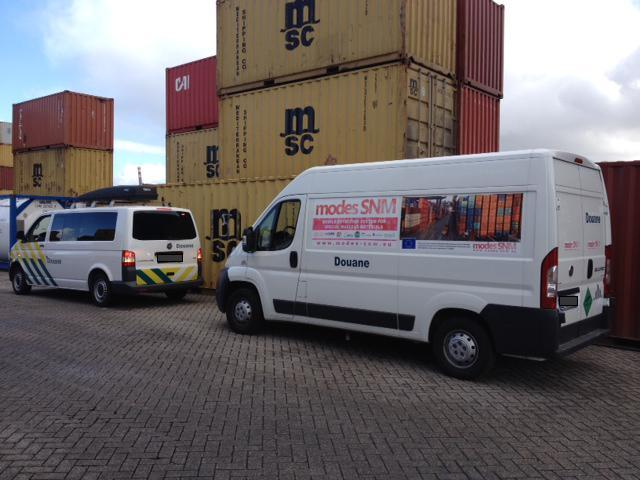
\includegraphics[width=110mm]{./Chapter7/figures/rotterdamContainers2.jpg}
\end{center}
\caption{The MODES van probing containers at the port while in motion.}
\label{fig:rotterdamContainers2}
\end{figure}
 
Radioactive tests were performed with some weak sources placed on a tripod $\sim$1 m away from the van with the side door closed. With van speeds of 10 km/h MODES was able to identify a $^{133}$Ba source, 0.45 MBq. AmBe was also identified but only when the van was slowed to 5 km/h, after a 60 s exposure yielded shielded neutron source. After this it was removed from the lead shield and a further identification gave AmBe and $^{241}$Am sources. The neutron rate recorded was 1.5 Hz, with a gamma alarm of 1400 Hz.
 
\begin{figure}
\begin{center}
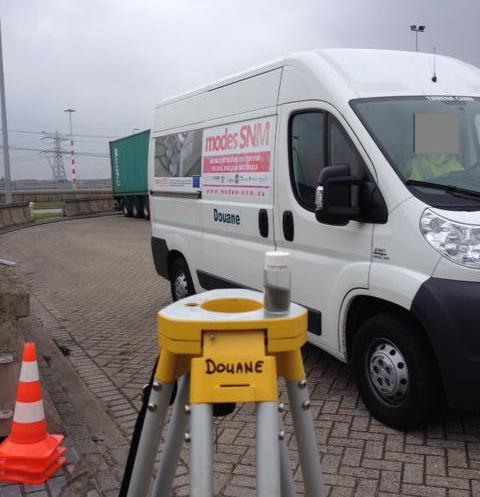
\includegraphics[width=100mm,height=100mm]{./Chapter7/figures/rotterdamTripodTest.jpg}
\end{center}
\caption{The MODES van being tested in mobile mode with known radioactive test samples on a tripod.}
\label{fig:rotterdamTripod}
\end{figure}

The system also suffered from many alarms when no containers were present, similar to as in Heathrow tests. Another problem encountered is the wifi connection with the system, as many times the connection would be lost and needed to be restarted. This was much more frequent than at Heathrow but is most likely due to the fact the door was closed for the testing at Rotterdam, whereas at Heathrow the door was left open, avoiding Faraday cage effects.

\subsection{Dublin Port Demonstration}
The port of Dublin is the largest port in Ireland. MODES was also deployed here to be used in conjunction with an X-ray scanning operation at the Coastal compound at the port. The MODES system was deployed in stationary mode $\sim$50 m from the 6 MeV mobile X-ray scanner (Nuctech). At this distance the MODES system did not experience any interference. The scanner is pictured in figure \ref{fig:dublinXRayScanner}.
 
\begin{figure}
\begin{center}
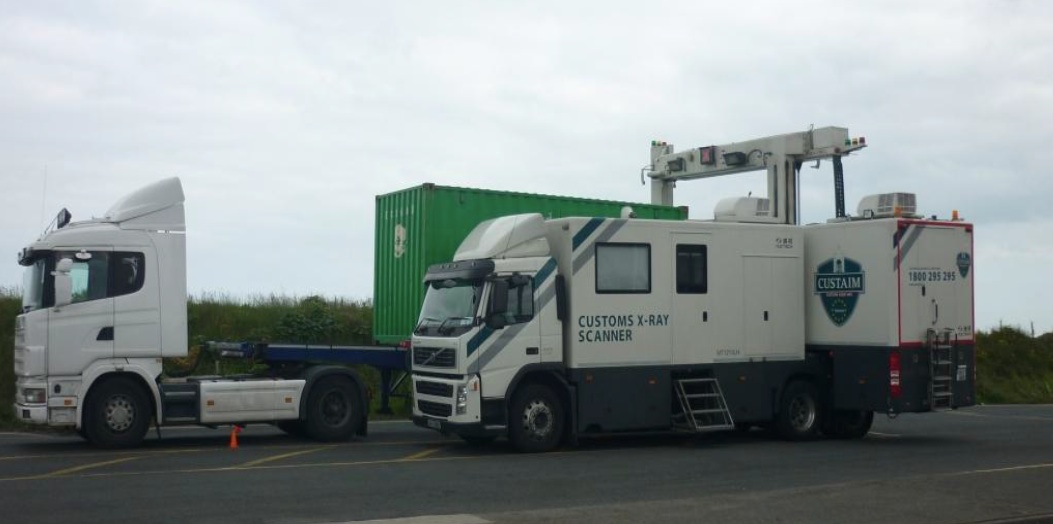
\includegraphics[width=100mm]{./Chapter7/figures/dublinXRayScanner1.jpg}
\end{center}
\caption{The Nuctech X-ray scanner used at the Dublin Port.}
\label{fig:dublinXRayScanner}
\end{figure}

In stationary operation a total of 83 containers and vehicles with cargo were scanned by the MODES system and no alarms were raised in them passing, however several alarms were raised when none were present. Two known containers of NORM were probed and raised an alarm both times in coherence with the X-ray scanner. These two cases of gamma alarms were triggered by containers holding ceramic tiles and clay pots. While both containers had been profiled as containing NORM, MODES yielded an erroneous identification of AmBe for the clay pots. 

It was also used in mobile operation to probe 60 containers but all failed to trigger an alarm. In absence of high traffic at the port the van was taken to the University College Dublin (UCD) to test against a Pu/Be source (37 GBq). The source was heavily sealed by tantalum and stainless steel capsules, containing 16 g of $^{239}$Pu oxide mixed with beryllium
metal. The source was held in a paraffin-filled drum, 0.51 m in height and 0.36 m in diameter. The drum was placed in a van and driven past the MODES system, at a speed of 8 km/h at $\sim$1 m away. This was increased to 4 m and the speed to 20 km/h, on both occasions the MODES system triggered gamma, neutron and thermal neutron alarms.

\subsection{Switzerland Field Tests}
Two locations in Switzerland were chosen for live field tests, the first at the Swiss border in Basel and the second at a Heavy Goods Traffic Center in Uri. These were the concluding  tests for the demonstration period.

\subsection{Swiss Customs, Basel}
At the Swiss Customs, Basel, the MODES system was setup in stationary mode and was used as a primary detector along side the Swiss Customs mobile X-ray scanner. Vehicles passing the border, pass both systems at speeds of $\sim$8 km/h. 38 vehicles were scanned over a period of 6 hours, no alarms were triggered. The background rate was measured at between 1.8 and 2.0 kHz, which fell to 1.2 - 1.5 kHz when vehicles passed the system, due to vehicle shielding.

\begin{figure}
\begin{center}
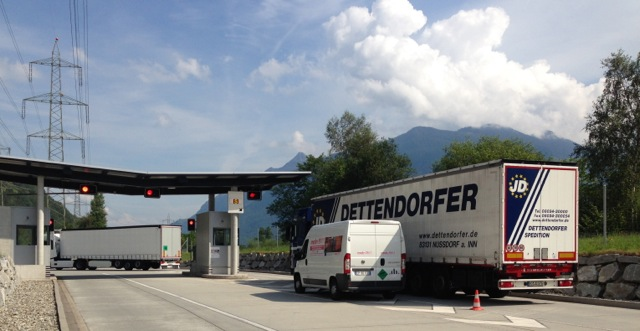
\includegraphics[width=100mm]{./Chapter7/figures/swissDemoPic1.jpg}
\end{center}
\caption{The MODES prototype system scanning at the Swiss Customs, Basel.}
\label{fig:swissDemo}
\end{figure}

\subsection{Software Upgrade}
After the first Swiss test an upgrade was applied to the software, addressing some key issues that were raised during the previous demonstrations. These were:

\begin{itemize}
	\item False alarm rate higher than expected
	\item Occasional low power to some detector tubes
	\item Conflict of GUIs when accessing from different devices
	\item Lack of data export tools
	\item More user information, count rate as a function of time
	\item Better compatibility with mobile devices
\end{itemize}

A key upgrade was the inclusion of the count rate as a function of time, as fluctuations can be obvious to the user and it can be used to localise radioactive material on vehicles, figure \ref{fig:softwareUpgrade}.

\begin{figure}
\begin{center}
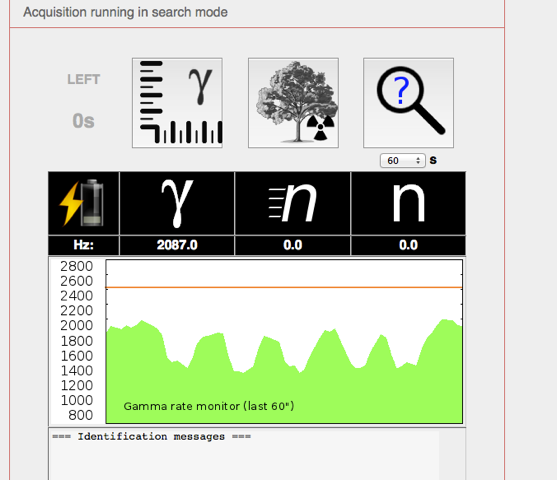
\includegraphics[width=100mm]{./Chapter7/figures/softwareUpdate.png}
\end{center}
\caption{The user interface after the software upgrade, showing count rate as a function of time. This example shows the background suppression when five trucks pass the system.}
\label{fig:softwareUpgrade}
\end{figure}

\subsection{Heavy Goods Traffic Centre, Uri}
Located in front of the Gotthard tunnel in Switzerland, the heavy goods traffic centre sees 1300-1500 trucks pass through every day. This is $\sim$75\% of all trucks driving through the Swiss border. The gamma background in Uri was twice the level of that in Basel, due to large amounts of Radon in Uri, with rates of $\sim$200-400 Bq/m$^{3}$ on average in this area, compared to $\sim$80-100 Bq/m$^{3}$ on average in Basel \cite{swissRadonLevels}.

Over a 2.5 hour window, 218 trucks were probed while the system was stationary. The speeds of the vehicles ranged from 5 - 25 km/h. No alarms occurred during this period, however 4 sharp peaks could be noticed, which involved short rapid increase in count rate, while no vehicles were present. These did not raise any false alarms due to the software upgrade.

\section{Summary}
The laboratory tests show the system meets the requirements of the IAEA and the demonstrations ultimately prove the durability, reliability and portability of the system. While traveling over 10,000 km across Europe the system, which was mounted in the van continuously over a period of 2 months, remained fully functional. It is also worth noting that the system traversed both land and sea on its journey. With the exception of wifi connection problems, the system worked without any major problems throughout the tests and each time it was easy to setup and use. Some key issues with the system were addressed before the final demonstration which most importantly removed the false alarm rate due to background fluctuations. Other issues still remain however with the need to extend the library to include medical isotopes persisting, as a lot of cargo transported via Heathrow involves medical isotopes.

For the majority of the demonstrations the system was deployed as a primary stationary detector, but ideally this system would be used as a secondary device. Although not tested as stringently as in primary mode, the demonstrations give an indication that this system is very capable of competing with current secondary devices.

The officials at each demonstration site were very impressed with the prototype. Many of the officials were especially keen on the simplicity and usability aspects of the system, with it very easy for non experts to use. They look forward to further developments from the system and retain close interest to its potential in the near future. 
